\begin{tikzpicture}[line cap=round,line join=round,scale=0.6]
\usetikzlibrary{calc}

% --- parameters (schematic) ---
\def\a{8.0}    % parabola y = -x^2 + a x
\def\bOne{12}  % y=b1 (top line)
\def\bTwo{6}   % y=b2 (middle line)
\def\bThree{2} % y=b3 (bottom line)

% helper: intersection x of -x^2 + a x = b  -> x = (a ± sqrt(a^2-4b))/2
\pgfmathsetmacro{\dOne}{sqrt(\a*\a-4*\bOne)}
\pgfmathsetmacro{\dTwo}{sqrt(\a*\a-4*\bTwo)}
\pgfmathsetmacro{\dThree}{sqrt(\a*\a-4*\bThree)}

\pgfmathsetmacro{\xoneL}{(\a-\dOne)/2}
\pgfmathsetmacro{\xoneR}{(\a+\dOne)/2}
\pgfmathsetmacro{\xtwoL}{(\a-\dTwo)/2}
\pgfmathsetmacro{\xtwoR}{(\a+\dTwo)/2}
\pgfmathsetmacro{\xthreeL}{(\a-\dThree)/2}
\pgfmathsetmacro{\xthreeR}{(\a+\dThree)/2}

% a point on the parabola below (for the oblique segment)
\coordinate (S) at (\xthreeL,\bThree); % treat as x3 on y=b3
\coordinate (T) at (\xoneL,\bOne);     % treat as x1 on y=b1

% --- draw the three horizontal lines ---
\draw[thick] (-0.2,\bOne) -- (\a+0.6,\bOne);
\draw[thick] (-0.2,\bTwo) -- (\a+0.6,\bTwo);
\draw[thick] (-0.2,\bThree) -- (\a+0.6,\bThree);

\node[right] at (\a+0.65,\bOne) {$y=b_1$};
\node[right] at (\a+0.65,\bTwo) {$y=b_2$};
\node[right] at (\a+0.65,\bThree) {$y=b_3$};

% --- parabola y = -x^2 + a x ---
\draw[thick] plot[domain=-0.2:\a+0.2,samples=200] (\x,{-(\x)*(\x)+\a*(\x)});
\node[right] at (\a-0.2,{-(\a-0.2)*(\a-0.2)+\a*(\a-0.2)}) {$y=-x^2+ax$};

% --- mark intersection points with labels x_i, y_i ---
\coordinate (X1) at (\xoneL,\bOne);
\coordinate (Y1) at (\xoneR,\bOne);
\coordinate (X2) at (\xtwoL,\bTwo);
\coordinate (Y2) at (\xtwoR,\bTwo);
\coordinate (X3) at (\xthreeL,\bThree);
\coordinate (Y3) at (\xthreeR,\bThree);

\foreach \P/\lab/\pos in {X1/$x_1$/above,Y1/$y_1$/above,X2/$x_2$/above,Y2/$y_2$/above,X3/$x_3$/below,Y3/$y_3$/below}{
  \fill (\P) circle (1.2pt);
  \node[\pos] at (\P) {\lab};
}

% --- the oblique segment (like the picture) from x3 to x1 ---
\draw[thick] (X3) -- (X1);

% --- label (x1+x3)/2 on the middle line (schematic position) ---
\pgfmathsetmacro{\xm}{(\xoneL+\xthreeL)/2}
\coordinate (M) at (\xm,\bTwo);
\fill (M) circle (1.1pt);
\node[below] at ($(M)+(0,-0.05)$) {$\dfrac{x_1+x_3}{2}$};

\end{tikzpicture}